\documentclass{notes}

\title{Discretisation of position and momentum}
\author{}

\usepackage{amssymb}
\usepackage{hyperref}
\usepackage[
    backend=biber,
    sorting=none,
    style=numeric-comp,
    citestyle=numeric-comp
]{biblatex}
\addbibresource{ref.bib}

\newcommand{\FVM}{\textsc{Fvm}}
\newcommand{\nRE}{n_{\rm RE}}
\newcommand{\Vp}{\mathcal{V}'}
\newcommand{\Jac}{\mathsf{J}}

\begin{document}
    \maketitle

    \noindent
    This document describes the (spatial/momentum) discretisations used in \DREAM.
    The overarching scheme used for deriving discretisations is the so-called
    finite-volume method (FVM).

    \tableofcontents

    \section{Grid definition}
    The most general grid used in \DREAM\ consists of three coordinates: one
    spatial coordinate $x$ and two momentum coordinates, $p_1$ and $p_2$. For
    a general coordinate $z^{(\alpha)}$, we introduce $N_\alpha$ cell grid points and
    $N_\alpha+1$ flux grid points and impose the definitions
    \begin{equation}
        \begin{aligned}
            \text{Flux grid:} & \qquad z^{(\alpha)}_{\rm min} = z^{(\alpha)}_{1/2} < z^{(\alpha)}_{3/2} < \ldots < z^{(\alpha)}_{N_\alpha+1/2} = z^{(\alpha)}_{\rm max},\\
            \text{Cell grid:} & \qquad z^{(\alpha)}_i = \frac{z^{(\alpha)}_{i+1/2} + z^{(\alpha)}_{i-1/2}}{2}, \quad (1\leq i \leq N_\alpha)\\
            &\qquad \Delta z^{(\alpha)}_i = z^{(\alpha)}_{i+1/2} - z^{(\alpha)}_{i-1/2}, \quad (1\leq i \leq N_\alpha)\\
            &\qquad \Delta z^{(\alpha)}_{i-1/2} = z^{(\alpha)}_i - z^{(\alpha)}_{i-1},\quad (2\leq i \leq N_\alpha).
        \end{aligned}
    \end{equation}

    \section{Boundary conditions}
    This section describes the various boundary conditions used in the code.
    In momentum space, the internal boundary conditions can be described from
    the distribution function symmetry relations
    \begin{equation}\label{eq:fsymmetry}
        \begin{aligned}
            f(-p,\theta) &= f(p,\pi-\theta),\\
            f(p,-\theta) &= f(p,\theta).
        \end{aligned}
    \end{equation}

    \subsection{Boundary conditions on $p/\xi$ grids}
    From the first of the symmetry relations~\eqref{eq:fsymmetry}, we find that
    that the flux through $p=0$ along a given pitch direction must be equal on
    both sides, implying that
    \begin{equation}
        \Phi^{(p)}\left(p=0^+, \xi\right) = \Phi^{(p)}\left(p=0^-, -\xi\right).
    \end{equation}

    From the second of the symmetry relations~\eqref{eq:fsymmetry}, we
    immediately find that the fluxes across the $\xi=\pm1$ boundaries vanish,
    i.e.\
    \begin{equation}\label{eq:bc:xiInternal}
        \Phi^{(\xi)}(p, \xi=1) = \Phi^{(\xi)}(p, \xi=-1) = 0.
    \end{equation}

    For external boundary conditions, we need to consider two cases. In the
    first case, the region above $p=p_{\rm max}$ is modelled as a fluid, and we
    thus only count the radial density $\nRE$ of runaway electrons. This
    means that we must count the flux through the $p=p_{\rm max}$ boundary, so
    that
    \begin{equation}
        \frac{\partial \nRE}{\partial t} =
        \int_{-1}^1 \Phi^{(p)}\left(p_{\rm max}, \xi\right)\,\frac{\Vp(r,p_{\rm max},\xi)}{V'(r)}\,\dd\xi.
    \end{equation}
    To evaluate $\Phi^{(p)}(p_{\rm max},\xi)$, which results from a combination
    of advection and diffusion on the momentum grid, we generally need to know
    the distribution function $f$ on both sides of $p=p_{\rm max}$. Since we do
    not keep track of $f$ above $p=p_{\rm max}$, we will need handle this in a
    special way. For the advection term, we simply set the interpolation
    coefficient $\delta_{N_p+1} = 0$, so that only the value of $f$ in
    $p=p_{N_p-1/2}$ is used. This could potentially cause problems with
    the preservation of positivity, and \red{we might want to consider other
    methods in the future.} For the diffusion term, however, no such simple fix
    exists, and we instead choose to interpolate in the flux:
    \begin{equation}
        \begin{aligned}
            \Phi^{(p)}_{N_p-1/2} &= \Phi^{(p)}_{N_p+1/2} - \Delta p_{N_p}\Phi^{\prime(p)}_{N_p+1/2},\\
            \Phi^{(p)}_{N_p-3/2} &= \Phi^{(p)}_{N_p+1/2} - (\Delta p_{N_p}+\Delta p_{N_p-1})
            \Phi^{\prime(p)}_{N_p+1/2},
        \end{aligned}
    \end{equation}
    where $\Phi^{\prime(p)} = \partial\Phi^{(p)}/\partial p$. Solving for
    $\Phi^{(p)}_{N_p+1/2}$ we obtain
    \begin{equation}
        \Phi^{(p)}_{N_p+1/2} = \Phi^{(p)}_{N_p-1/2} +
        \frac{\Delta p_{N_p}}{\Delta p_{N_p-1}} \left( \Phi^{(p)}_{N_p-1/2} - \Phi^{(p)}_{N_p-3/2} \right).
    \end{equation}

    In the second case, when the runaway grid is enabled, we want the flux
    across the hot-tail $p=p_{\rm max}$ to enter (or leave) the runaway grid
    seamlessly. If the hot-tail and runaway grids have the same $\xi$ grids,
    this is rather straightforward as we simply set 
    $\Phi^{(p)}_{\rm hot}(p_{\rm max},\xi) = \Phi^{(p)}_{\rm RE}(p_{1/2},\xi)$.
    However, in \DREAM, we allow for the two grids to be different (we only
    enforce $p^{\rm RE}_{1/2} = p^{\rm hot}_{\rm max}$) and so we must connect
    the two grids in some way. To conserve particles, we require that the
	number of particles added to the runaway (RE) grid are also removed from
	the hot-tail grid. Specifically,
	\begin{equation}\label{eq:fluxCross_origin}
		\begin{gathered}
			-\int \left[\nabla\cdot\bb{\Phi}\right]^{\rm RE}_{1,J}\,\Vp^{\rm RE}_{1,J}\dd p\,\dd\xi =
			\int \left[\nabla\cdot\bb{\Phi}\right]^{\rm hot}_{N_p,j}\,\Vp^{\rm hot}_{N_p,j}\dd p\,\dd\xi,\\
			\implies\\
			%
			-\sum\frac{\Vp^{\rm RE}_{1/2,J}\Phi^{\rm RE}}{\Vp^{\rm RE}_{1,J}\Delta p^{\rm RE}_1}\Vp^{\rm RE}_{1,J}\Delta p^{\rm RE}_1 \Delta\xi^{\rm RE}_J =
			\sum_j\frac{\Vp^{\rm hot}_{N_p+1/2,j}\Phi^{\rm hot}}{\Vp^{\rm hot}_{N_p,j}\Delta p^{\rm hot}_{N_p}}\Vp^{\rm hot}_{N_p,j}\Delta p^{\rm hot}_{N_p}\Delta\xi^{\rm hot}_{j}, % \overline{\Delta\xi}_{jJ},
		\end{gathered}
	\end{equation}
    As we will see in section~\ref{sec:discr:adv:bc}, in \DREAM\ we specify the
    flux of particles on the hot-tail grid, and then enforce the flux on the
    runaway grid by requiring that the flux into each cell is
    \begin{equation}\label{eq:fluxCross}
        \Phi^{\rm RE}(p_{1/2},\xi_J) \Vp^{\rm RE}_{1/2,J} \Delta^{\rm RE}_J =
        -\sum_j \Phi^{\rm hot}\left(p_{\rm max},\xi_j\right) \Vp^{\rm hot}_{N_p+1/2,j} \overline{\Delta\xi}_{jJ},
    \end{equation}
	where $\overline{\Delta\xi}_{jJ}$ is
    \begin{equation}\label{eq:PhiPinterp}
        \overline{\Delta\xi}_{jJ,\rm hot} = \min\left(\xi_{J+1/2,{\rm hot}},\xi_{j+1/2,{\rm RE}}\right) -
        \max\left( \xi_{J-1/2,{\rm hot}}, \xi_{j-1/2,{\rm RE}} \right),
    \end{equation}
    so that $\Delta\xi_{j,\rm RE} = \sum\overline{\Delta\xi}_{jJ,\rm hot}$, and
	the sum is taken over all $j$ such that $\xi_j\in[\xi_{J-1/2}, \xi_{J+1/2}]$.
	%Simplifying equation~\eqref{eq:fluxCross_origin} we obtain the relation
    %\begin{equation}\label{eq:fluxCross}
    %    -\Phi^{\rm RE}(p_{1/2},\xi_J)\Vp^{\rm RE}_{1/2,J}\Delta\xi^{\rm RE}_{J} =
    %    \sum_{j} \Phi^{\rm hot}(p_{\rm max},\xi_J) \Vp^{\rm hot}_{N_p+1/2,j} \overline{\Delta\xi}_{jJ},
    %\end{equation}
	%which must be satisfied for the particle number to be conserved across the
	%two grids.

    \section{Spatial discretisations}
    In this section we describe the various discretisations used in \DREAM. We
    however begin by describing the general approach taken to discretising
    equations in the code.

    \subsection{Finite volume method}
    In order to achieve mass conservation, we use the finite-volume method to
    discretise our equations and consider the fluxes between cells on the
    computational grid. For a general flux-conservative term
    $\nabla\cdot\bb{\Phi}$, we take the matrix row corresponding to element
    $i_1\cdots i_D$ ($D$ being the problem dimensionality) of the unknown
    quantity to be
    \begin{equation}
        \left[ \nabla\cdot\bb{\Phi} \right]_{i_1\cdots i_D}  =
            \frac{1}{\Vp_{i_1\cdots i_D}}\sum_\beta \frac{
                \Phi^{(\beta)}_{i_\beta+1/2} \Vp_{i_\beta+1/2} -
                \Phi^{(\beta)}_{i_\beta-1/2} \Vp_{i_\beta-1/2}
            }{\Delta z^{(\beta)}_{i_\beta}},
    \end{equation}
    where $\Vp$ denotes the phase space Jacobian, Greek indices denote the
    coordinate (i.e.\ $z_\alpha, z_\beta, \ldots$), Latin indices denote grid
    points and the matrix indices which are not shifted have been suppressed for
    clarity (i.e.\
    $\Phi^{(\beta)}_{i_\beta+1/2}\equiv\Phi^{(\beta)}_{i_1\cdots i_\beta+1/2\cdots i_D}$).

    \subsection{Advection term}\label{sec:advection}
    A general advection term can be written on the form
    \begin{equation*}
        \nabla\cdot\left( \bb{F} f \right),
    \end{equation*}
    with $\bb{F} = \zhat^{(\alpha)}F^{(\alpha)} + \zhat^{(\beta)}F^{(\beta)}+\ldots$
    denoting the advection coefficient and $f$ the distribution function. For
    momentum-space friction, we discretise such terms according to
    \begin{equation}\label{eq:advection:discr}
        \left[\nabla\cdot\left( \bb{F}f \right) \right]_{i_1\cdots i_D} =
            \frac{1}{\Vp_{i_1\cdots i_D}}\sum_\beta \frac{
                F^{(\beta)}_{i_\beta+1/2}f_{i_\beta+1/2} \Vp_{i_\beta+1/2} -
                F^{(\beta)}_{i_\beta-1/2}f_{i_\beta-1/2} \Vp_{i_\beta-1/2}
            }{\Delta z^{(\beta)}_{i_\beta}},
    \end{equation}
    Since the distribution function is only known on the cell grid, but is here
    required on the flux grid, we must interpolate. We may interpolate linearly in
    $f$ according to
    \begin{equation}
        f_{i_\beta-1/2} = \delta^{(\beta)}_{i_\beta} f_{i_\beta} + \left( 1 - \delta^{(\beta)}_{i_\beta} \right) f_{i_\beta-1},
    \end{equation}
    where the interpolation coefficients $\delta^{(\beta)}_{i_\beta}$ are
    determined with the help of any of the methods described in
    section~\ref{sec:interp}. (Note that unnecessary indices have been
    suppressed, so that really
    $\delta^{(\beta)}_{i_\beta} = \delta^{(\beta)}_{i_1\cdots i_\beta\cdots i_D}$).
    
    DREAM more generally supports interpolation via a general 4-point stencil according to
    \begin{equation}
        f_{i_\beta-1/2} = \sum_{k=0}^3 \delta^{(\beta)}_{i_\beta,k} f_{i_\beta-2+k}.
    \end{equation}
    

    \subsubsection{Boundary conditions on $p/\xi$ grid}\label{sec:discr:adv:bc}
    Internal boundary conditions at $p=p_{1/2}$ must be specified explicitly.
    They must then be inserted appropriately into~\eqref{eq:advection:discr} so
    that
    \begin{equation}
        \left[ \nabla\cdot\left( \bb{F}f \right) \right]_{1,j} = \frac{
            \Vp_{3/2} F_{3/2}^{(p)} f_{3/2} - \Vp_{1/2}\Phi^{(p)}_{1/2}
        }{\Delta p_{1}}
    \end{equation}
    where $\Phi_{1/2}^{(p)}$ is the phase space particle flux into or out of
    the inner boundary. At $\xi=\xi_{1/2}$ and $\xi=\xi_{N_\xi+1/2}$, however,
    we use the result~\eqref{eq:bc:xiInternal} and obtain (for the $\xi$ term)
    \begin{equation}
        \begin{aligned}
            \left[ \nabla\cdot\left( \bb{F} f \right) \right]_{i,1} &=
                \frac{\Vp_{3/2} F^{(\xi)}_{i,3/2} f_{i,3/2}}{\Delta\xi_{1}},\\
            %
            \left[ \nabla\cdot\left( \bb{F} f \right) \right]_{i,N_\xi} &=
                -\frac{\Vp_{N_\xi-1/2} F^{(\xi)}_{i,N_\xi-1/2} f_{i,N_\xi-1/2}}{\Delta\xi_{N_\xi}}.
        \end{aligned}
    \end{equation}

    \paragraph{Combining kinetic grids}
    When combining the hot-tail and runaway grids, we want the particles to flow
    seamlessly from one grid to another across their shared boundary. This is
    not automatically guaranteed, since the hot-tail and runaway grids need not
    have the same resolutions and so cell may overlap arbitrarily. The only
    property we can be certain that the grids satisfy is that
    $p_{N_p+1/2}^{\rm hot} = p_{1/2}^{\rm RE}$. To achieve a seamless flow of
    particles between the grids, we first write out the discretized forms of the
    boundary fluxes on each grid:
    \begin{equation}\label{eq:crossCondition}
        \begin{aligned}
            \left[ \nabla\cdot\left( \bb{F}f \right)\right]^{\rm hot}_{N_p,j} &=
                \frac{\Vp^{\rm hot}_{N_p+1/2}\Phi^{\rm hot}_j - \Vp_{N_p-1/2} F_{N_p-1/2}f_{N_p-1/2}}{\Delta p^{\rm hot}_{N_p}},\\
            \left[ \nabla\cdot\left( \bb{F}f \right)\right]^{\rm RE}_{1,J} &=
                \frac{\Vp^{\rm RE}_{3/2} F^{(p)}_{3/2} f_{3/2,J} - \Vp^{\rm RE}_{1/2}\Phi^{\rm RE}_J}{\Delta p^{\rm RE}_1},
        \end{aligned}
    \end{equation}
    where $\Phi^{\rm hot}$ and $\Phi^{\rm RE}$ denote the fluxes into the
    hot-tail and runaway grids respectively. According to the usual recipe used
    in a finite volume discretization, the hot-tail flux $\Phi^{\rm hot}_j$
    should be given by
    \begin{equation}
        \Phi^{\rm hot}_j = F_{N_p+1/2,j}^{\rm hot} f_{N_p+1/2,j}^{\rm hot}.
    \end{equation}
    However, the hot-tail distribution is only known in integer grid points with
    $i\leq N_p$, and so to evaluate $f_{N_p+1/2,j}^{\rm hot}$ we must
    interpolate. In contrast to the usual situation, we however have two
    different distribution functions on each side of the cell face on which the
    flux is to be evaluated. We therefore write the flux grid distribution as
    \begin{equation}
        f_{N_p+1/2,j}^{\rm hot} = \delta^{(1)}_{j}f_{N_p,j} +
            \left( 1-\delta^{(1)}_{j} \right) \hat{f}^{\rm RE}_j,
    \end{equation}
    where $\delta^{(1)}$ is an interpolation coefficient (to be determined)
    and $\hat{f}^{\rm RE}_j$ is a function of the RE distribution function in
    the cells adjacent to cell $j$ on the hot-tail grid. Various possibilities
    for choosing $\hat{f}^{\rm RE}_j$ can be foreseen, but here we decide to
    use the rather straightforward
    \begin{equation}
        \hat{f}^{\rm RE}_j = \delta^{(2)}_j f^{\rm RE}_{J_j} +
            \left( 1 - \delta^{(2)}_j \right) f^{\rm RE}_{J_j-1},
    \end{equation}
    where $\delta^{(2)}_j$ is an interpolation coefficient and $J_j$ is the
    first $J$ such that $\xi^{\rm RE}_{J_j}\geq\xi^{\rm hot}_j$ (if $J_j=1$,
    (index 0 in C++) we set $\delta^{(2)}_j = 1$). With this form for the
    runaway distribution function, we obtain the flux grid distribution value
    \begin{equation}
        f^{\rm hot}_{N_p+1/2,j} = \delta^{(1)}_j f_j^{\rm hot} +
            \left( 1 - \delta^{(1)}_j \right)\left[
                \delta^{(2)}_j f_{J_j}^{\rm RE} +
                \left( 1-\delta^{(2)}_{J_j} \right) f_{J_j-1}^{\rm RE}
            \right].
    \end{equation}
    Next, we must choose the interpolation coefficients $\delta^{(1)}_j$ and
    $\delta^{(2)}_j$. For any type of advection, a desirable property of the
    interpolation coefficients is to preserve the monotonicity of the
    distribution function. Unfortunately it would be rather difficult to use
    the general flux limiter scheme otherwise available in \DREAM, but to still
    have some protection against oscillations we use an up-wind interpolation
    scheme:
    \begin{equation}
        \delta^{(1)}_j = \begin{cases}
            1, \quad&\text{if } F_{N_p+1/2}^{\rm hot} \leq 0,\\
            0, \quad&\text{otherwise}.
        \end{cases}
    \end{equation}
    For the second interpolation coefficient, we use a linear interpolation in
    $\xi$. This is known to generally be prone to oscillations for pure
    advection problems, but in our situation the problem may be significantly
    helped by the pitch-angle diffusion present which can often be stronger
    than the $\xi$-component of the electric field in the region of interest
    (near $\xi\sim1$):
    \begin{equation}
        \begin{gathered}
            \hat{f}^{\rm RE}_j = f^{\rm RE}_{J_j} +
                \left( \xi^{\rm hot}_j - \xi^{\rm RE}_{J_j-1} \right)
                \frac{f_{J_j}^{\rm RE} - f_{J_j-1}^{\rm RE}}
                {\xi^{\rm RE}_{J_j} - \xi^{\rm RE}_{J_j-1}} \implies\\
                %
                \delta^{(2)}_j = \frac{\xi^{\rm hot}_j - \xi^{\rm RE}_{J_j-1}}
                {\xi^{\rm RE}_{J_j} - \xi^{\rm RE}_{J_j-1}}.
        \end{gathered}
    \end{equation}
    Again, when $J_j=1$ (index 0 in C++), we let $\delta^{(2)}_j = 1$.

    For the flux on the runaway grid, we use equation~\eqref{eq:fluxCross}
    directly to ensure the conservation of density.

    \subsubsection{Boundary conditions on $p_\parallel / p_\perp$ grid}
    \emph{To be written...}

    \subsection{Diffusion term}\label{sec:diffusion}
    A general diffusion term can be written on the form
    \begin{equation*}
        \nabla\cdot\left( \mathbb{D}\cdot\nabla f \right),
    \end{equation*}
    where $\mathbb{D}$ is the diffusion tensor
    \begin{equation*}
        \mathbb{D} = \begin{pmatrix}
            D_{rr} & D_{r1} & D_{r2} \\
            D_{1r} & D_{11} & D_{12} \\
            D_{2r} & D_{21} & D_{22}
        \end{pmatrix}.
    \end{equation*}
    In \DREAM, we neglect the radial cross-terms, i.e.\
    $D_{r1} = D_{1r} = D_{r2} = D_{2r} = 0$.

    For the diffusion term, we will need to approximate derivatives of the
    distribution function $f$. For the diagonal terms (i.e.\ the $D_{rr}$,
    $D_{11}$ and $D_{22}$ terms), this is straightforward: since the derivatives
    should be evaluated on the flux grid, we can use a basic central difference
    approximation:
    \begin{align}
        \left.\frac{\partial f}{\partial r}\right|_{k-1/2,i,j} &=
            \frac{f_{k,i,j} - f_{k-1,i,j}}{\Delta r_{k-1/2}},\\
        %
        \left.\frac{\partial f}{\partial p_1}\right|_{k,i-1/2,j} &=
            \frac{f_{k,i,j} - f_{k,i-1,j}}{\Delta p_{1; i-1/2}},\\
        %
        \left.\frac{\partial f}{\partial p_2}\right|_{k,i,j-1/2} &=
            \frac{f_{k,i,j} - f_{k,i,j-1}}{\Delta p_{2; j-1/2}},\\
    \end{align}
    Since no interpolation in $f$ is needed, these terms automatically preserve
    the positivity of the solution.

    The cross terms cause some problems with preservation of positivity.
    Unfortunately we cannot use the same interpolation scheme as for the
    advection term. To easily support the use of diffusion cross terms, we
    therefore use simple cell averaging, which does \emph{not} preserve
    positivity. We write the derivatives as
    \begin{equation}
        \begin{aligned}
            \left.\frac{\partial f}{\partial p_1}\right|_{k,i,j-1/2} &=
                \frac{f_{i+1,j} + f_{i+1,j-1} - f_{i-1,j} - f_{i-1,j-1}}
                {\Delta p_{1;i+1/2} + \Delta p_{1;i-1/2}},\\
            %
            \left.\frac{\partial f}{\partial p_2}\right|_{k,i-1/2,j} &=
                \frac{f_{i,j+1} + f_{i-1,j+1} - f_{i,j-1} - f_{i-1,j-1}}
                {\Delta p_{2;j+1/2} + \Delta p_{2;j-1/2}}.
        \end{aligned}
    \end{equation}
    If we would like to also preserve positivity, we should instead use the
    approach taken by refs.~\cite{DuToit2018,Daniel2019}. They rewrite the
    diffusion cross terms as advection terms, which allows us to use the same
    methods as in section~\ref{sec:advection}. The ``advection form'' for the
    diffusion cross terms is
    \begin{equation}
        \begin{aligned}
            \left[ D_{12}\frac{\partial f}{\partial p_2} \right] &=
                \frac{\partial (\ln f)}{\partial p_2}D_{12} f = \tilde{D}_{12} f,\\
            %
            \left[ D_{21}\frac{\partial f}{\partial p_1} \right] &=
                \frac{\partial (\ln f)}{\partial p_1}D_{21} f = \tilde{D}_{21} f,
        \end{aligned}
    \end{equation}
    where we have introduced the modified diffusion coefficients
    $\tilde{D}_{12}\equiv D_{12}\partial(\ln f)/\partial p_2$ and
    $\tilde{D}_{21}\equiv D_{21}\partial(\ln f)/\partial p_1$. These modified
    diffusion coefficients depend on (non-linearly) on the unknown, and hence
    they require a non-linear solver. We choose not to implement this form of
    the diffusion coefficients directly in the \DREAM/\FVM\ library, but instead
    refer to the physicist to rewriting her equations according to the above
    and implement them using the advection term class instead.

    \paragraph{Full discretisation}
    Within the framework of the finite-volume method, we discretise the general
    diffusion term as
    \begin{equation}
        \begin{aligned}
            \left[ \nabla\cdot\left( \mathbb{D}\cdot\nabla f \right) \right]_{kij} &=
                \frac{1}{\Vp_{i_1\cdots i_D}}\Bigg[\\
                %
                &\frac{1}{\Delta r_k}\left(
                    \Vp_{k+1/2}D_{rr;k+1/2}\frac{f_{k+1,i,j}-f_{k,i,j}}{\Delta r_{k+1/2}} -
                    \Vp_{k-1/2}D_{rr;k-1/2}\frac{f_{k,i,j}-f_{k-1,i,j}}{\Delta r_{k-1/2}}
                \right) +\\
                %
                &+ \frac{1}{\Delta p_{1;i}} \left(
                    \Vp_{i+1/2}D_{11;i+1/2}\frac{f_{k,i+1,j} - f_{k,i,j}}{\Delta p_{1;i+1/2}} -
                    \Vp_{i-1/2}D_{11;i-1/2}\frac{f_{k,i,j} - f_{k,i-1,j}}{\Delta p_{1;i-1/2}}
                \right) +\\
                %
                &+ \frac{1}{\Delta p_{2;i}} \left(
                    \Vp_{j+1/2}D_{22;j+1/2}\frac{f_{k,i,j+1} - f_{k,i,j}}{\Delta p_{2;j+1/2}} -
                    \Vp_{j-1/2}D_{22;j-1/2}\frac{f_{k,i,j} - f_{k,i,j-1}}{\Delta p_{2;j-1/2}}
                \right) +\\
                %
                &+ \Vp_{i+1/2}D_{12;i+1/2}\frac{
                    f_{k,i+1,j+1} + f_{k,i,j+1} - f_{k,i+1,j-1} - f_{k,i,j-1}
                }{\Delta p_{1;i}\left(\Delta p_{2;j+1/2} + \Delta p_{2;j-1/2} \right)} -\\
                &- \Vp_{i-1/2}D_{12;i-1/2}\frac{
                    f_{k,i,j+1} + f_{k,i-1,j+1} - f_{k,i,j-1} - f_{k,i-1,j-1}
                }{\Delta p_{1;i}\left(\Delta p_{2;j+1/2} + \Delta p_{2;j-1/2} \right)} +\\
                %
                &+ \Vp_{j+1/2}D_{21;j+1/2}\frac{
                    f_{k,i+1,j+1} + f_{k,i+1,j} - f_{k,i-1,j+1} - f_{k,i-1,j}
                }{\Delta p_{2;j}\left(\Delta p_{1;i+1/2} + \Delta p_{1;i-1/2} \right)} -\\
                &- \Vp_{j-1/2}D_{21;j-1/2}\frac{
                    f_{k,i+1,j} + f_{k,i+1,j-1} - f_{k,i-1,j} - f_{k,i-1,j-1}
                }{\Delta p_{2;j}\left(\Delta p_{1;i+1/2} + \Delta p_{1;i-1/2} \right)}\\
            &\Bigg].
        \end{aligned}
    \end{equation}

	\subsubsection{Boundary conditions on $p/\xi$ grid}

    \paragraph{On combined kinetic grids}
    When combining hot-tail and runaway grids, we use a similar discretization
    for the diffusion flux as for the advection flux described above. With the
    same choice for $\hat{f}^{\rm RE}_j$ as above we have
    \begin{equation}
        \left.\frac{\partial f^{\rm hot}}{\partial p}\right|_{N_p+1/2,j} =
            \frac{f^{\rm hot}_j - \delta^{(2)}_j f_{J_j}^{\rm RE} -
            \left( 1 - \delta^{(2)}_j \right) f^{\rm RE}_{J_j-1}}
            {p^{\rm RE}_{1/2} - p^{\rm hot}_{N_p+1/2}}.
    \end{equation}

    \section{Interpolating in distribution function}\label{sec:interp}
    In advection terms, as well as diffusion cross terms, we must evaluate the
    distribution function on the flux grid. Since the distribution function is
    only explicitly computed on the cell grid, this means that we must
    interpolate in the distribution function. A simple scheme is provided by 
    linear interpolation, for which one can generally write
    \begin{equation}
        f_{i-1/2} = \delta_{i} f_i + \left( 1 - \delta_i \right) f_{i-1}.
    \end{equation}
    In the simplest approach with uniform grids, we take $\delta_i\equiv 1/2$, making $f_{i-1/2}$
    a simple average of the value of $f$ in the adjacent cells. While simple and
    often accurate enough, other schemes for choosing $\delta_i$ can provide
    better stability and even desirable physical properties such as preservation
    of positivity. These schemes are referred to as ``flux limiter schemes'',
    and we also provide those in the code.
    
    For additional flexibility and accuracy, we consider general 4-point stencils of the form
    \begin{equation}
    	f_{i-1/2} = \sum_{k=-2}^1 \delta^{(i)}_k f_{i+k}.
    \end{equation}
    In order to improve numerical stability and reduce oscillations, schemes with 
    upwind bias are advantageous where $\delta_{1}$ vanishes for positive 
    advection coefficients, and $\delta_{-2}$ for negative advection. In what follows,
    we will assume a positive advection coeffient $A_{i-1/2}>0$. For the $A_{i-1/2}<0$ 
    case, all interpolation coefficients will be mirrored, and can be obtained with the 
    mapping $k \mapsto -1 - k$.
    
    A general second-order accurate scheme can be generated from the so-called
    $\kappa$ schemes (given here for uniform grids, but are implemented more generally):
    \begin{align*}
    \delta_{-2} &= -\frac{1-\kappa}{4}, \nonumber \\
    \delta_{-1} &= 1 - \frac{\kappa}{2}, \nonumber \\
    \delta_0 &= \frac{1+\kappa}{4}, \nonumber \\
    \delta_1 &= 0.
    \end{align*}
    Here, $\kappa = 1$ corresponds to the linear interpolation (central difference) 
    scheme described above; since it has no upwind bias, it is less stable than other 
    $\kappa$ schemes. A common choice is $\kappa=0.5$ which yields the QUICK 
    scheme (which is the only choice of $\kappa$ that also gives third-order accuracy) 
    or $\kappa=-1$ which yields a purely upwind linear-extrapolation scheme (Second-order upwind).

    \subsection{Flux limiter schemes}
    The previous scheme, which is classified as linear since the interpolation 
    coefficients $\delta_k$ are independent of the solution, can be generalised to a 
    useful class of non-linear \emph{flux-limiter schemes}, which are given by
    (again specialising to uniform grids for compactness)
    \begin{align}
    \delta^{(i)}_{-2} &= -\frac{\psi(r^{(i)})}{2}, \nonumber \\
    \delta^{(i)}_{-1} &= 1 + \frac{\psi(r^{(i)})}{2}, \nonumber \\
    \delta^{(i)}_{0} &= 0, \nonumber \\
    \delta^{(i)}_{1} &= 0, \nonumber \\
    r^{(i)} &= \frac{f_i - f_{i-1}}{f_{i-1}-f_{i-2}}.
    \end{align}
    Via the function $\psi(r)$, the interpolation coefficients depend non-linearly on 
    the distribution $f$. Although it is not explicitly written on that form, the linear $\kappa$ schemes 
    are exactly retrieved with $\psi(r) = (1+\kappa)r/2 + (1-\kappa)/2$ (by comparing the net $f_{i-1/2}$ 
    obtained after interpolating). It can be shown that positivity preservation (or the more strict condition 
    of \emph{boundedness}, where $f_{i-1} \leq f_{i-1/2} \leq f_i$)
    will be satisfied by letting $\psi$ obey certain constraints.
    
    Three flux limiters that are implemented in DREAM are:
    \begin{align}
    \psi(r) &= \text{max}(0,\,\text{min}(2r,\,(1+3r)/4,\,4)), && \text{(SMART)} \nonumber \\
    \psi(r) &= \text{max}(0,\,\text{min}(2r,\,(1+r)/2,\,2)), && \text{(MUSCL)} \nonumber \\
    \psi(r) &= \frac{3}{2}\frac{r(1+r)}{r^2+r+1}. && \text{(OSPRE)}
    \end{align}
    For Dreicer generation, all three flux limiters give comparable accuracy, but OSPRE is the 
    more robust one thanks to its continuous form. 
    In some situations, convergence of the piece-wise flux limiters may be accelerated (or restored)
    by under-relaxing the algorithm, which we do by updating
    \begin{align}
    \delta = \delta_\text{prev} + \eta [\delta_\text{calc} - \delta_\text{prev}],
    \end{align}
    where $\eta \in [0,1]$ is a damping factor, $\delta_\text{calc}$ the interpolation coefficient
    according to the scheme chosen and $\delta_\text{prev}$ the coefficient in the previous iteration 
    of the non-linear solver. Sometimes a value of $\eta \approx 0.9$ is sufficient -- too low
    values can prevent convergence altogether.
    
    The accuracy of the interpolation schemes are compared in figure \ref{fig:advection interpolation convergence}.
    The first-order upwind scheme is outside of view as it significantly overpredicts the generation. Computation times 
    are not indicated, but the linear 2-point stencils Centered and UPWIND are fastest, then the linear 3-point stencils 
    QUICK and second-order upwind (UPWIND-2), and finally the flux limiters which are all significantly slower since 
    they require the non-linear solver to be used.
    
    \begin{figure}
    \begin{center}
    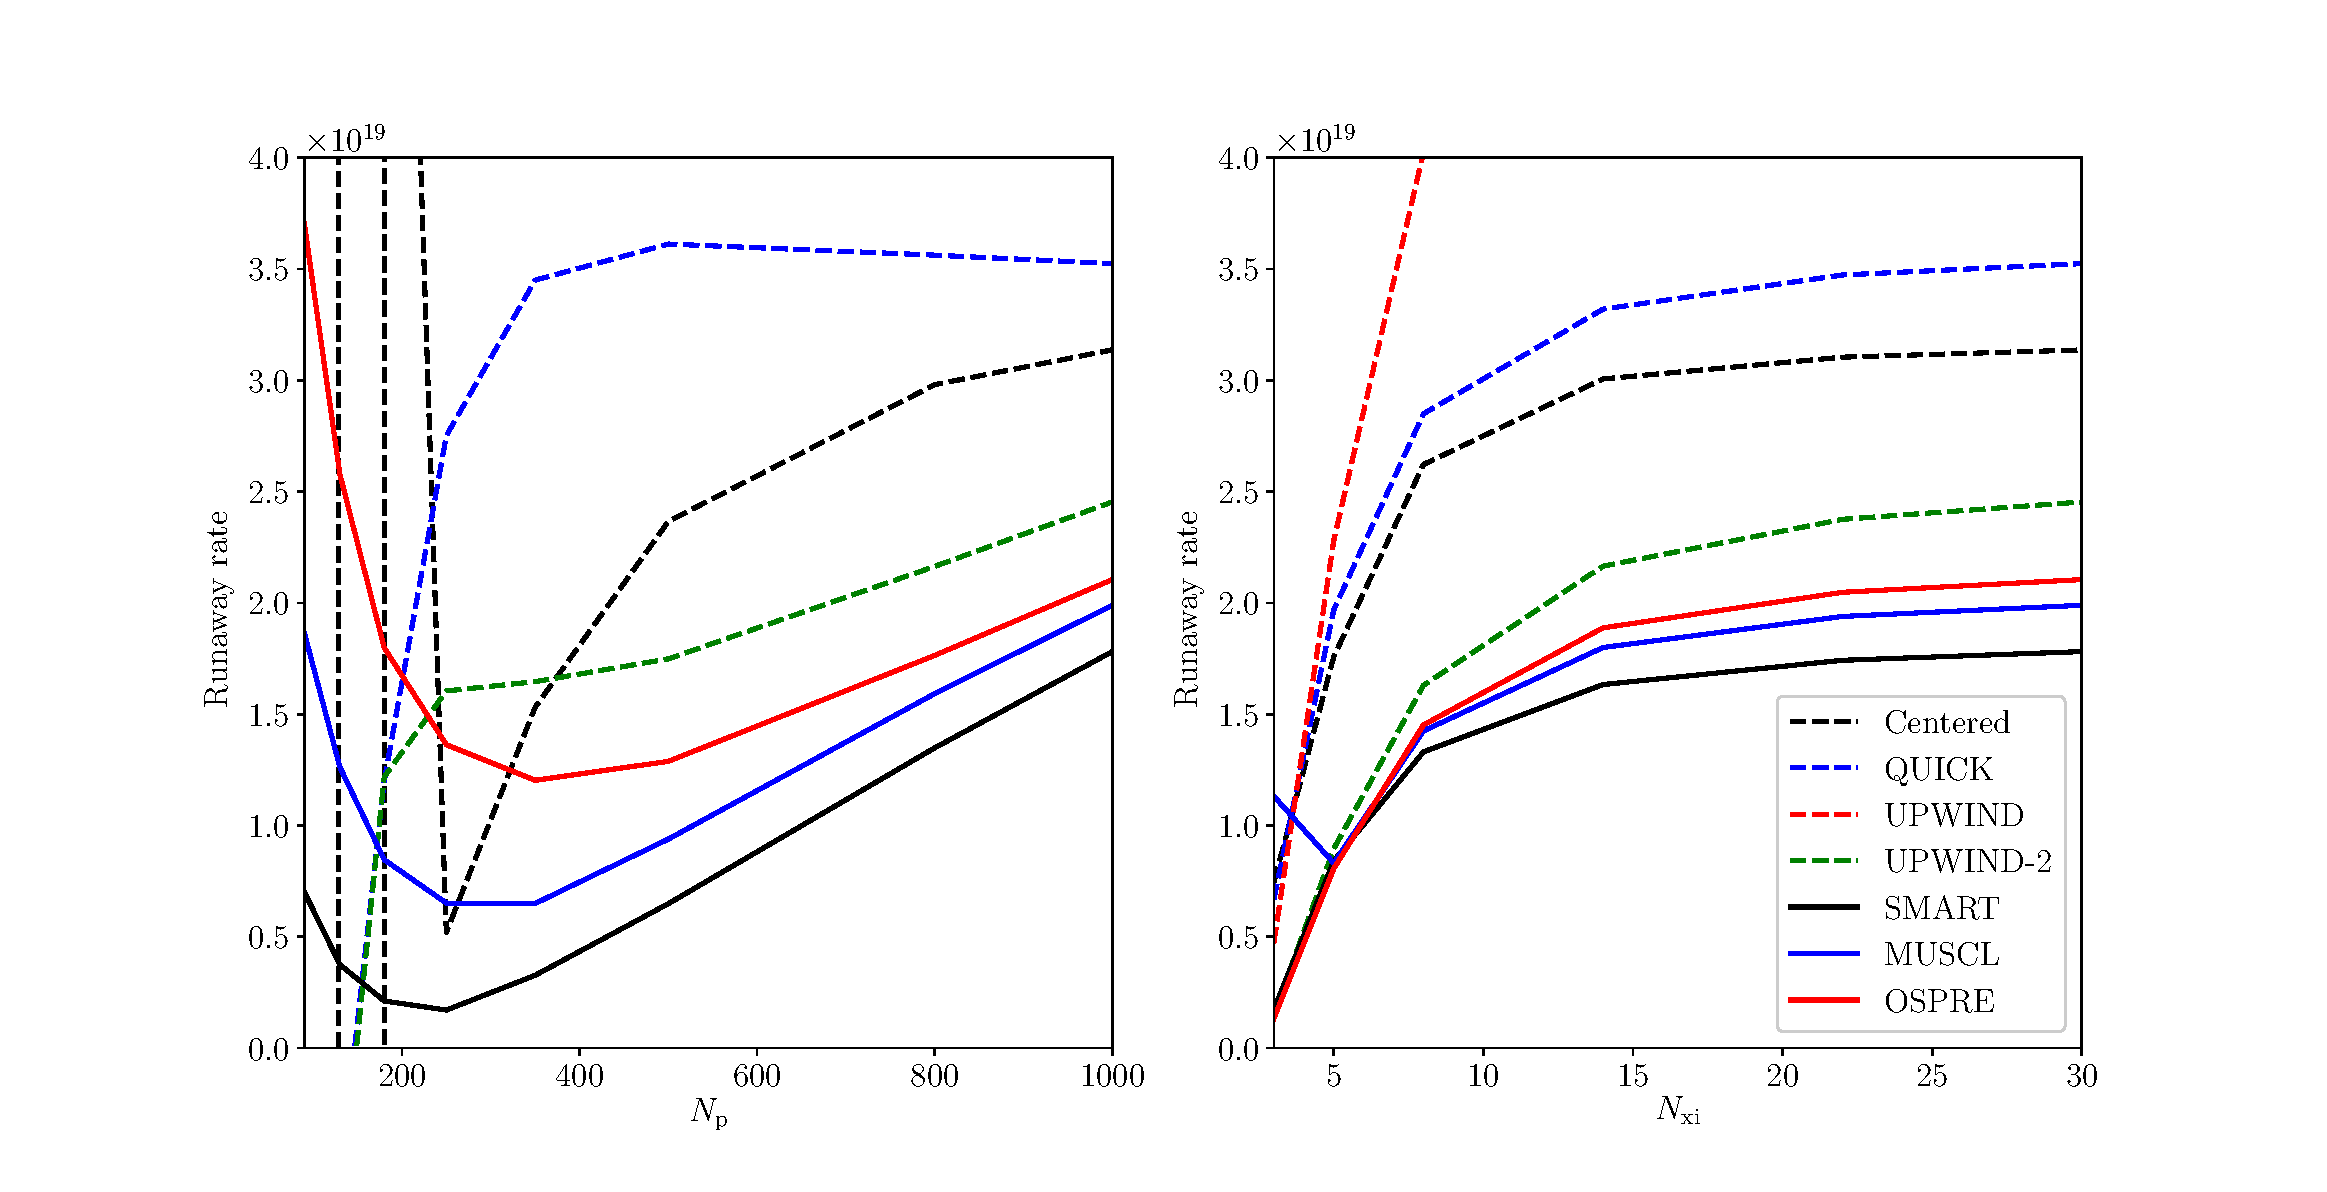
\includegraphics[width=1.0\textwidth,trim=25mm 0 25mm 0]{advection_interpolation_convergence}
    \caption{\label{fig:advection interpolation convergence} Runaway rate $\partial n_\mathrm{RE}/\partial t$ in 
    a basic Dreicer runaway scenario with parameters: $n_e = 5\times 10^{19}\,$m$^{-3}$, $T_e = 100\,$eV, $Z=1$, 
    $E=6.74546\,$V/m, run for $t_\mathrm{max}=1$\,ms in 10 time steps, with a grid extending to 
    $p_\mathrm{max} = 2m_e c$ with boundary condition $f(p_\mathrm{max})=0$ .}
    \end{center}
    \end{figure}
    \section{Solution of non-linear system}
    The set of equations we aim to solve can generally be formulated as the
    root-finding problem,
    \begin{equation}\label{eq:nonlinear}
        \bb{F}(\bb{x}) = 0,
    \end{equation}
    where $\bb{F}$ represents the physical equations to solve. A number of
    approaches could be imagined for solving this equation, and in this section
    we will review those implemented in \DREAM.

    \subsection{Linearly implicit solution}
    The linearly implicit solution method relies on the slow time evolution of
    the system in question. Let us assume that $\bb{F}$ may be decomposed into
    \begin{equation}
        \bb{F}\left( \bb{x} \right) = M\left( \bb{x} \right) \bb{x} + S\left( \bb{x} \right)
    \end{equation}
    where $M$ takes the form of a linear operator which may depend non-linearly
    on $\bb{x}$, and $S$ takes the form of a source term. In a linearly implicit
    scheme, one assumes that $M$ and $S$ depend weakly on $\bb{x}$, thus
    justifying the approximation
    \begin{equation}
        \bb{F}\left( \bb{x}_{n+1} \right)\approx M\left( \bb{x}_n\right) \bb{x}_{n+1}
        + S\left( \bb{x}_n \right).
    \end{equation}
    In this approximation, equation~\eqref{eq:nonlinear} may be solved by
    inverting the matrix $M$:
    \begin{equation}
        \bb{x}_{n+1} = M^{-1}\left(\bb{x}_n\right) S\left(\bb{x}_n\right).
    \end{equation}
    In contrast to the more accurate Newton method, the linearly implicit scheme
    requires no iteration, and thus only one matrix inversion. This can make the
    scheme beneficial for evolving systems which vary slowly in time.
    
    \subsection{Newton's method}
    The more general \emph{Newton's method} is obtained by Taylor expanding
    equation~\eqref{eq:nonlinear} around $\bb{x}^{(k+1)} = \bb{x}^{(k)} + \Delta\bb{x}$:
    \begin{equation}
        \bb{F}\left( \bb{x}^{(k+1)} \right)\approx \bb{F}\left(\bb{x}^{(k)}\right) +
        \Jac\left(\bb{x}^{(k)}\right) \left( \bb{x}^{(k+1)} - \bb{x}^{(k)} \right) = 0.
    \end{equation}
    Here, $\Jac(\bb{x}^{(k)}) = \partial\bb{F}(\bb{x}^{(k)})/\partial\bb{x}$
    denotes the Jacobian matrix of $\bb{F}$. Solving for $\bb{x}^{(k+1)}$, we
    obtain the iterative scheme
    \begin{equation}
        \bb{x}^{(k+1)} = \bb{x}^{(k)} - \Jac^{-1}\left( \bb{x}^{(k)} \right) \bb{F}\left( \bb{x}^{(k)} \right),
    \end{equation}
    which hopefully converges to the true zero of $\bb{F}$. Here, we thus rely
    on a series of iterations to obtain the true solution in any given time
    step.

    The most difficult part of Newton's method is evaluating the Jacobian
    $\Jac$.

    \addcontentsline{toc}{section}{References}
    \printbibliography

\end{document}

